\section{Results}
\subsection{Capabilities and label budgets favor different towers}
\label{sec:profiles}
Table~\ref{tab:capability} shows capability profiles without an aggregate score.
DINOv2 has the highest measured depth, normal, and NAVI performance, while Muse Glimmer
has the highest full-label recognition estimate and the lowest tower-stage scores on
all three correspondence datasets. These are observed levels; most cross-tower pairs
have not been tested with intervals.

\begin{table}[t]
\centering\small
\caption{Capability profiles. Recognition uses the label-budget runs at 1\% and 100\%,
with final-layer features and the matched attention readout. Depth and normals are the best observed matched test scores across sampled
layers, not independently validated layer selections. NAVI uses the final layer.
Retention is accuracy at 50\% occlusion divided by clean accuracy. Higher is better except
for normals. No overall rank is assigned.}
\label{tab:capability}
\begin{tabular}{lrrrrrr}
\toprule
Tower & 1\% labels & Full labels & Depth $\uparrow$ & Normals $\downarrow$ & NAVI $\uparrow$ & Retention\\
\midrule
DINOv2 & 0.3689 & 0.9079 & 0.7015 & 18.85 & 0.5389 & 0.5194\\
SigLIP2 & 0.6559 & 0.9168 & 0.6702 & 23.90 & 0.4013 & 0.4883\\
Muse Glimmer & 0.4330 & 0.9212 & 0.6588 & 24.30 & 0.2139 & 0.5163\\
Kimi K2.6 & 0.3448 & 0.8862 & 0.6595 & 25.51 & 0.3646 & 0.2786\\
Qwen3.8 & 0.2451 & 0.8791 & 0.6736 & 24.24 & 0.3785 & 0.3046\\
Kimi K3 & 0.2191 & 0.8369 & 0.6546 & 27.03 & 0.3334 & 0.2042\\
\bottomrule
\end{tabular}

\end{table}

Three full-label recognition comparisons have paired intervals in the matched attention
arm. Muse Glimmer exceeds DINOv2 by $0.0125$ $[0.0034,0.0215]$ top-1. Muse Glimmer versus
SigLIP2, $0.0041$ $[-0.0036,0.0121]$, and SigLIP2 versus DINOv2,
$0.0084$ $[-0.0009,0.0178]$, remain unresolved. The data therefore do not establish a
unique full-label recognition winner.

The label budget changes the observed ordering (Figure~\ref{fig:labels}). With one
training image per class, SigLIP2 reaches 0.6559 top-1, compared with Muse Glimmer's
0.4330. At full labels their estimates converge to 0.9168 and 0.9212. Qwen3.8's nominal
1\% cell is unstable: its seed standard deviation is 0.0780 around a mean of 0.2451.
These curves describe label efficiency under the pooled attention readout, whose
full-token control remains inconclusive.

\begin{figure}[t]
\centering
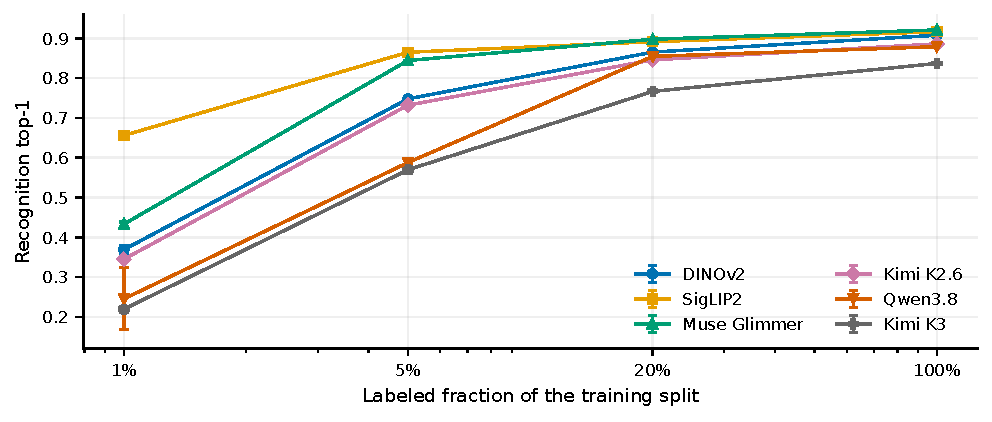
\includegraphics[width=\textwidth]{figures/paper-label-budget.pdf}
\caption{Recognition across label budgets at the final tower layer, matched attention arm.
Points average three seeds; vertical bars show one seed standard deviation, not confidence
intervals. The nominal 1\% budget contains 100 images.}
\label{fig:labels}
\end{figure}

Two cross-tower geometry comparisons were rerun with deterministic PCA at layers
selected from the test-score sweep, without independent validation of that selection. DINOv2 exceeds
Qwen3.8 in depth by $0.0292$ $[0.0099,0.0484]$ $\delta_1$, but that comparison also
changes native grid size from $28\times28$ to $32\times32$. DINOv2 reduces normal error
relative to SigLIP2 by $5.0370$ $[4.3038,5.8164]$ degrees; both use $32\times32$ grids.
These intervals support the named comparisons under their protocols, not a complete
geometry ranking.

Occlusion adds another distinction. At 50\% masking, DINOv2, Muse Glimmer, and SigLIP2
retain approximately half their clean accuracy, compared with 20--31\% for the other
three towers. This grouping is descriptive: available occlusion intervals compare clean
and perturbed images within a stage, not retention between towers.
Appendix~\ref{app:secondary} gives the curves and stage-level interpretation.

\subsection{Geometry usually peaks before the final layer}
\label{sec:layers}
Across two capacity arms, geometry has a pre-final test-score peak in 23 of 24
combinations of tower, task, and capacity arm. The exception is DINOv2 depth in the raw arm.
Recognition reaches its highest score at the final layer in 19 of 24 combinations of
tower, readout, and arm. Figure~\ref{fig:layers} shows attention recognition, depth, and
normals for both arms; Appendix~\ref{app:peaks} lists the geometry peaks.

In the matched arm, choosing the final layer instead of the best observed layer reduces
depth $\delta_1$ by 0.0256--0.1422 and increases normal error by 4.34--10.22 degrees.
These are descriptive sweep differences: the peak was identified on the same test
scores being compared, and intervals were not computed for every peak-to-final contrast.
The result motivates validating intermediate layers for spatial tasks. It does not
establish a universal optimal fraction of tower depth.

\begin{figure}[t]
\centering
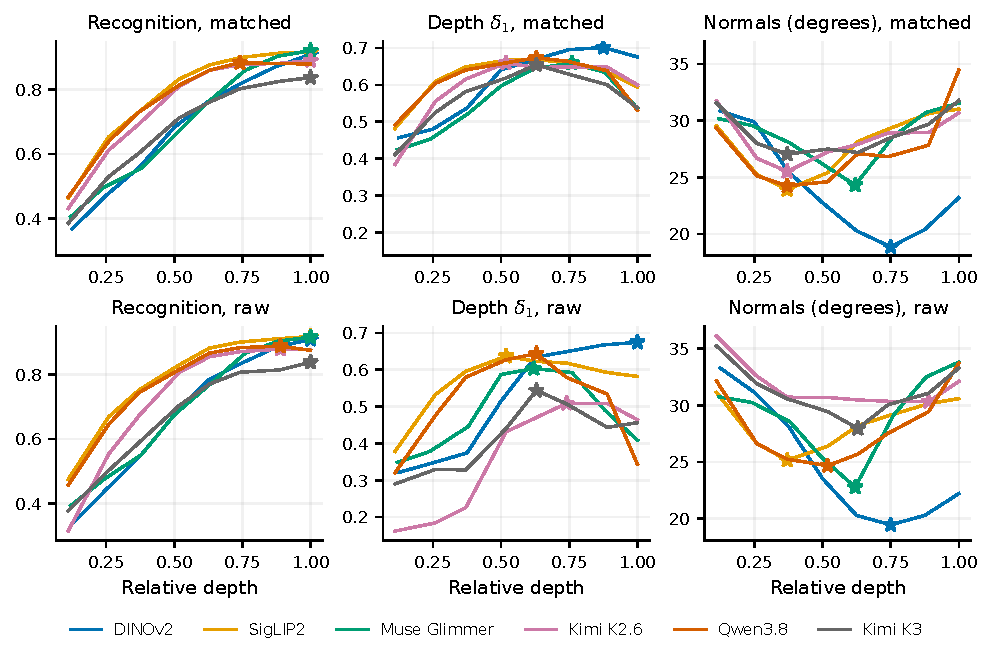
\includegraphics[width=\textwidth]{figures/paper-layers.pdf}
\caption{Layer sweeps at the tower stage. Columns show recognition with attention pooling,
DIODE depth, and DIODE normals; rows show matched and raw arms. Stars mark each curve's
best observed test score. Recognition uses pooled tokens; geometry uses full patch grids.
Matched geometry curves come from the original randomized-PCA sweep.}
\label{fig:layers}
\end{figure}

Qwen3.8 accounts for four recognition curves whose peak is earlier than the final layer;
Kimi K2.6 raw attention accounts for the fifth. Qwen3.8's earlier-layer advantage resolves
in raw attention, $0.0128$ $[0.0053,0.0203]$, and raw mean,
$0.0156$ $[0.0053,0.0263]$. Its two matched comparisons cross zero. The nominal Kimi
K2.6 decline is smaller than its seed standard deviation and was not tested with an
interval. Thus even this exception depends on the readout and capacity setting.

\subsection{Connector effects change across evaluations}
\label{sec:projectors}
We expected the connector to reduce spatial recoverability. DIODE gives the opposite
pattern: all 16 projected-versus-final-tower comparisons favor projected features, and
15 paired intervals exclude zero. These comprise four connectors, two geometry tasks,
and two capacity arms. The unresolved comparison is Kimi K2.6 raw depth,
$0.0196$ $[-0.0003,0.0402]$ $\delta_1$.

\begin{figure}[t]
\centering
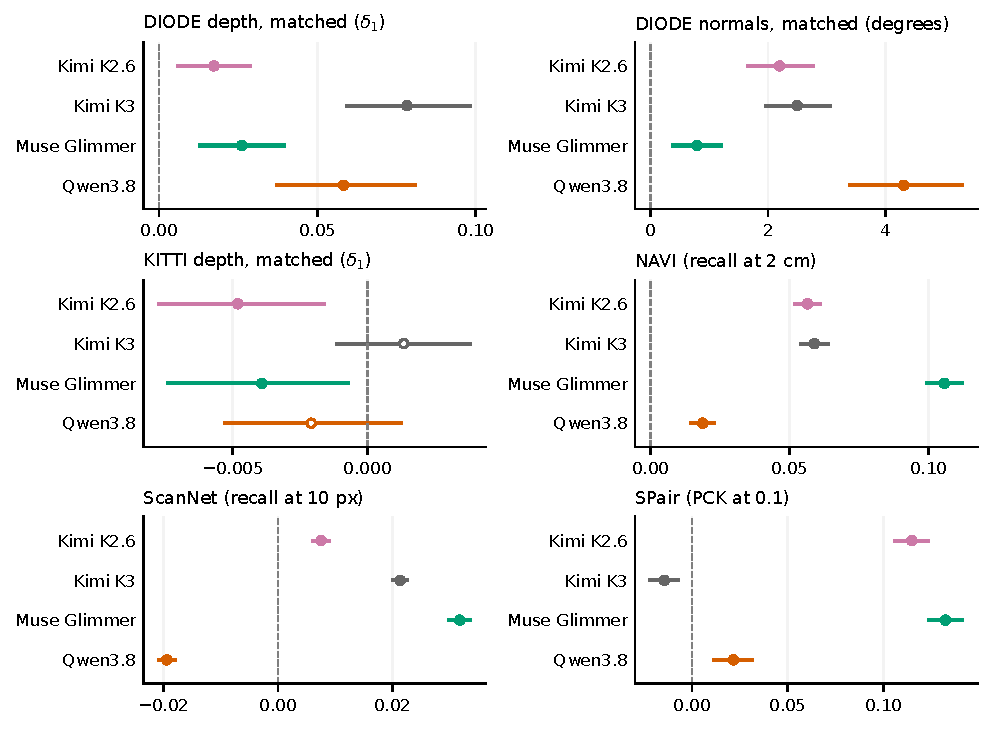
\includegraphics[width=\textwidth]{figures/paper-projectors.pdf}
\caption{Projected features versus final tower features. Positive favors projected;
for normals the difference is tower error minus projected error. DIODE and KITTI panels
use matched readouts; correspondence is training-free. Bars are paired 95\% intervals,
with open markers where they cross zero. Each panel has its own metric and scale.
Appendix~\ref{app:intervals} includes both geometry arms and exact values.}
\label{fig:projectors}
\end{figure}

The matched DIODE gains range from 0.0174 to 0.0784 in depth $\delta_1$ and from
0.7924 to 4.3130 degrees of normal-error reduction. The largest raw depth gain is
Qwen3.8's 0.1601, compared with 0.0584 after capacity matching. Because PCA also changes
the input representation, the difference between arms is a sensitivity result rather
than an isolated estimate of the effect of head size.

On KITTI, Kimi K2.6 and Muse Glimmer reverse: projected-minus-tower differences are
$-0.0048$ $[-0.0077,-0.0016]$ and $-0.0039$ $[-0.0074,-0.0007]$ $\delta_1$, respectively.
Kimi K3 and Qwen3.8 are unresolved. Training new readouts on driving scenes therefore
does not reproduce the uniformly positive DIODE pattern. The datasets differ in scene
content, target coverage, depth range, and sample size; this study does not isolate
which difference causes the reversal.

Correspondence yields ten positive and two negative intervals, all excluding zero.
Qwen3.8's projected-minus-tower difference is $+0.0188$ $[0.0146,0.0230]$ on NAVI but
$-0.0194$ $[-0.0208,-0.0180]$ on ScanNet. Kimi K3's SPair difference is
$-0.0144$ $[-0.0216,-0.0070]$, while both geometric correspondence differences are positive. SPair compares
parts across different object instances, so this result concerns a different capability
from NAVI's same-object multiview consistency.

\subsection{Lossless merging exposes readout sensitivity}
\label{sec:merge}
A stage score can change even when the transformation discards no information.
On NAVI, Qwen3.8 scores 0.3785 at the tower stage, 0.1130 after merging, and 0.3973 after
projection. Merging concatenates neighboring tokens; it changes the vectors compared by
cosine matching and their spatial sampling. The drop therefore cannot by itself establish
information loss. Kimi K2.6 and Muse Glimmer show the same drop-and-recovery pattern.

This control demonstrates sensitivity to representation format. It does not provide a
numerical bound on the portion of a projector effect attributable to that sensitivity.
Likewise, a trained depth probe can recover more from projected features without the
projector adding new image information. Throughout, the measured outcome is performance
under a particular readout and training procedure.
